\chapter{Experiment and Results}
\label{expt}
\section{Part A: Classification of the Cardiotocography dataset}
\label{part1}

The details of this dataset are as follows:
\begin{quote}
This project aims at building neural networks to classify the Cardiotocography dataset containing measurements of fetal heart rate (FHR) and uterine contraction (UC) features on 2126 cardiotocograms classified by expert obstetricians [1]. The dataset can be obtained from: https://archive.ics.uci.edu/ml/datasets/Cardiotocography.

The cardiotocograms were classified by three expert obstetricians and a consensus classification label with respect to a morphologic pattern and to a fetal state (N: Normal; S: Suspect; P: Pathologic) was assigned to each of them. The aim is to predict the N, S and P class labels in the test dataset after training the neural network on the training dataset.
\end{quote}

In this dataset, data is first split into a 70:30 ratio, then cross-validated using a 5 fold cross-validation. 

The definition of the 3 layer network as required by the question is shown in Listing \ref{ls:1_l3}, whereas the loss minimization and accuracy prediction is shown in Listing \ref{ls:1_loss}.

\begin{lstlisting}[language=Python, caption= Definition of a 3 layer network, label=ls:1_l3]
def l3_ffn(x, neuron_size, weight_decay_beta):
    """Feedforward net with 1 hidden layer
    """
    sum_regularization = 0
    with tf.name_scope('hidden'):
        weights = tf.Variable(tf.truncated_normal([NUM_FEATURES, neuron_size], stddev=1.0/math.sqrt(float(NUM_FEATURES))), name='weights')
        biases  = tf.Variable(tf.zeros([neuron_size]), name='biases')
        h  = tf.nn.relu(tf.matmul(x, weights) + biases)
        sum_regularization += weight_decay_beta * tf.nn.l2_loss(weights)
    with tf.name_scope('linear'):
        weights = tf.Variable(tf.truncated_normal([neuron_size, NUM_CLASSES], stddev=1.0/math.sqrt(float(neuron_size))), name='weights')
        biases  = tf.Variable(tf.zeros([NUM_CLASSES]), name='biases')
        u = tf.matmul(h, weights) + biases
        sum_regularization += weight_decay_beta * tf.nn.l2_loss(weights)
    
    return u, sum_regularization
\end{lstlisting}

\begin{lstlisting}[language=Python, caption= Definition of a 3 layer network, label=ls:1_loss]
x = tf.placeholder(tf.float32, [None, NUM_FEATURES])
y_ = tf.placeholder(tf.float32, [None, NUM_CLASSES])

if layers==3:
    logits, regularizer = l3_ffn(x, neuron_size, weight_decay)
elif layers == 4:
    logits, regularizer = l4_ffn(x, neuron_size, weight_decay)
else:
    print('Invalid number of layers given.')
    return

cost = tf.nn.softmax_cross_entropy_with_logits_v2(labels=y_, logits=logits)
loss = tf.reduce_mean(cost + regularizer)

# Create the gradient descent optimizer with the given learning rate.
optimizer = tf.train.GradientDescentOptimizer(learning_rate)
train_op = optimizer.minimize(loss)

correct_prediction = tf.cast(tf.equal(tf.argmax(logits, 1), tf.argmax(y_, 1)), tf.float32)
accuracy = tf.reduce_mean(correct_prediction)
\end{lstlisting}

Additionally the setup of a 5 fold cross-validation is shown in Listing \ref{ls:1_folds} and the handling of batches sizes are shown in Listing \ref{ls:1_batch_size}.

\begin{lstlisting}[language=Python, caption= 5 fold cross-validation, label=ls:1_folds]
num_folds = 5
for fold in range(num_folds):
    print(f'Fold number: {fold+1}')
    n = int(train_x.shape[0] / num_folds)
    fold_start, fold_end = fold*n, (fold+1)*n
    x_test, y_test = train_x[fold_start:fold_end], train_y[fold_start:fold_end]
    x_train  = np.append(train_x[:fold_start], train_x[fold_end:], axis=0)
    y_train = np.append(train_y[:fold_start], train_y[fold_end:], axis=0) 
\end{lstlisting}

\begin{lstlisting}[language=Python, caption= Batch size setup, label=ls:1_batch_size]
for start, end in zip(range(0, len(x_train), batch_size), range(batch_size, len(x_train), batch_size)):
    train_op.run(feed_dict={x: x_train[start:end], y_: y_train[start:end]})
\end{lstlisting}

Finally, the training results used in this experiment is assumed to be the ones obtained from cross-validation obtained from Listing \ref{ls:1_folds}, while the test set used are assumed to be the test set obtained from the initial 70:30 split from the original data.

\subsection{Question 1}
\label{1q1}
\begin{quote}
1. Design a feedforward neural network which consists of an input layer, one hidden layer of 10 neurons with ReLU activation function, and an output softmax layer. Assume a learning rate = 0.01, L2 regularization with weight decay parameter = $10^{-6}$, and batch size = 32. Use appropriate scaling of input features.

a) Use the training dataset to train the model and plot both accuracies on training and
testing data against epochs.

b) State the approximate number of epochs where the test error converges.
\end{quote}

\subsubsection{Part A}
The following plot in Figure \ref{fig:1a} is obtained for Q1a.
\begin{figure}[H]
    \centering
    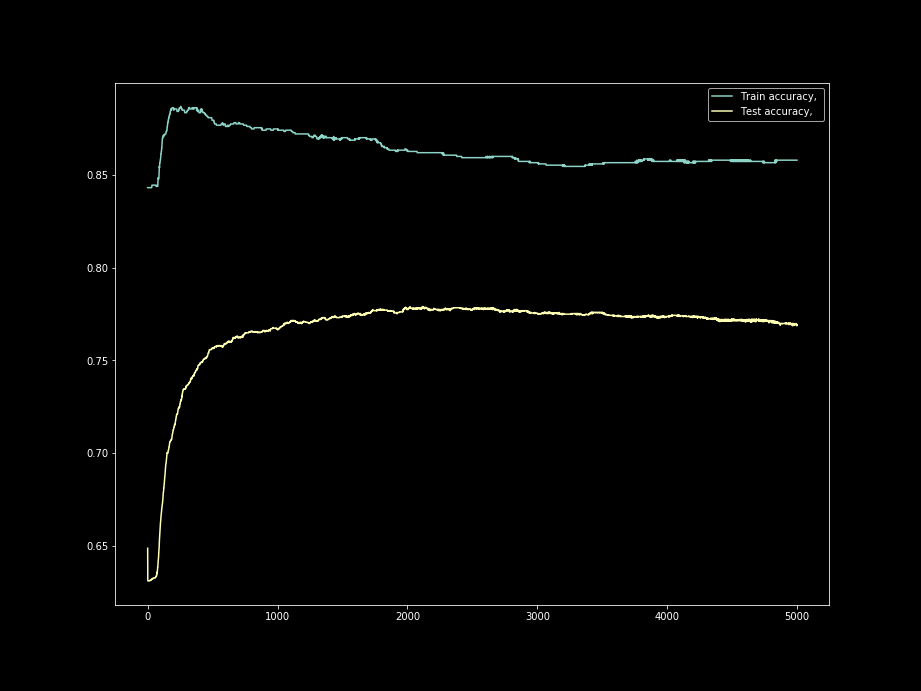
\includegraphics[width=0.8\linewidth]{assets/plots/part1_Q1a.png}
    \caption{Plot of training and testing data against epochs}
    \label{fig:1a}
\end{figure}

Some parameters used in this question are:
\begin{itemize}
    \item Learning Rate: 0.01
    \item Weight Decay Parameter: $10^{-6}$
    \item Batch Size: 32
\end{itemize}

\subsubsection{Part B}
The approximate number of epochs where test errors converges is 2000 as the trend can be seen to plateau around that point in Figure \ref{fig:1a}. While the end of the curve actually does reduce after more epochs, the general trend still has a gradient of 0.

\subsection{Question 2}
\label{1q2}
\begin{quote}
2. Find the optimal batch size by training the neural network and evaluating the performances for different batch sizes.

a) Plot cross-validation accuracies against the number of epochs for different batch sizes. Limit search space to batch sizes {4, 8, 16, 32, 64}. Plot the time taken to train the network for one epoch against different batch sizes.

b) Select the optimal batch size and state reasons for your selection.

c) Plot the train and test accuracies against epochs for the optimal batch size.

 Note: use this optimal batch size for the rest of the experiments.
\end{quote}

\subsubsection{Part A}
\begin{figure}[H]
    \begin{subfigure}{1\textwidth}
        \centering
        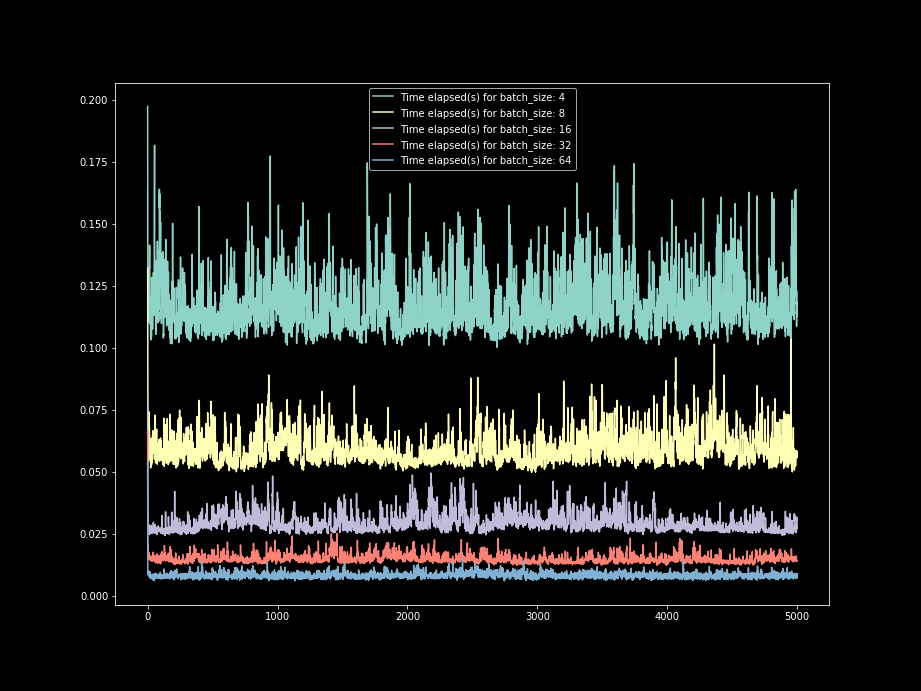
\includegraphics[width=0.8\linewidth]{assets/plots/part1_Q2a_1.png}
        \caption{Time taken for one epoch for different batch sizes}
        \label{fig:batch_time}
    \end{subfigure}
\end{figure}
\begin{figure}[H]
    \ContinuedFloat
    \begin{subfigure}{1\textwidth}
        \centering
        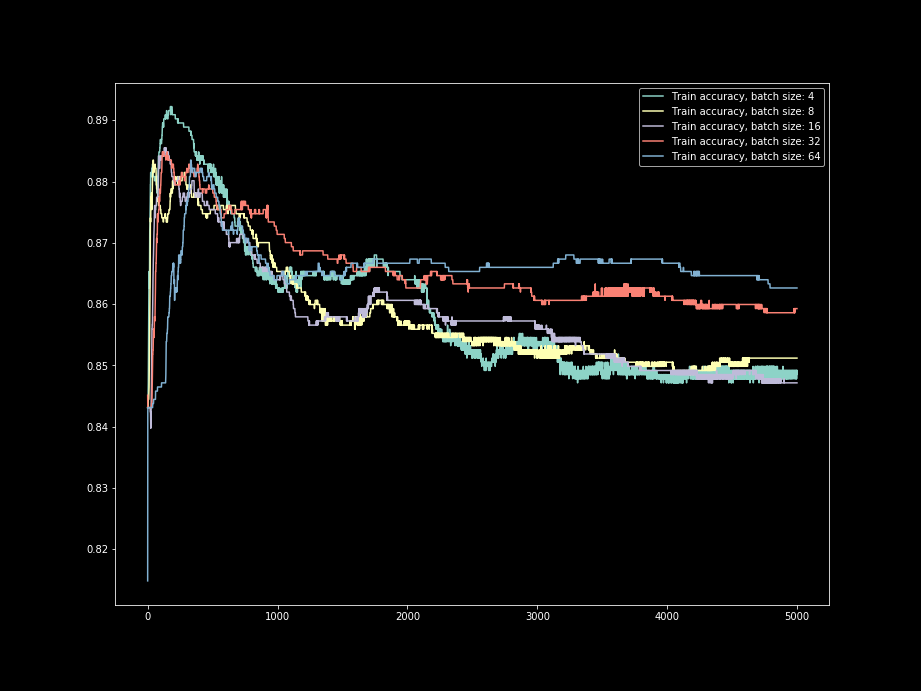
\includegraphics[width=0.8\linewidth]{assets/plots/part1_Q2a_4.png}
        \caption{Training accuracy for different batch sizes}
        \label{fig:train_batch}
    \end{subfigure}
\end{figure}
\begin{figure}[H]
    \ContinuedFloat
    \begin{subfigure}{1\textwidth}
        \centering
        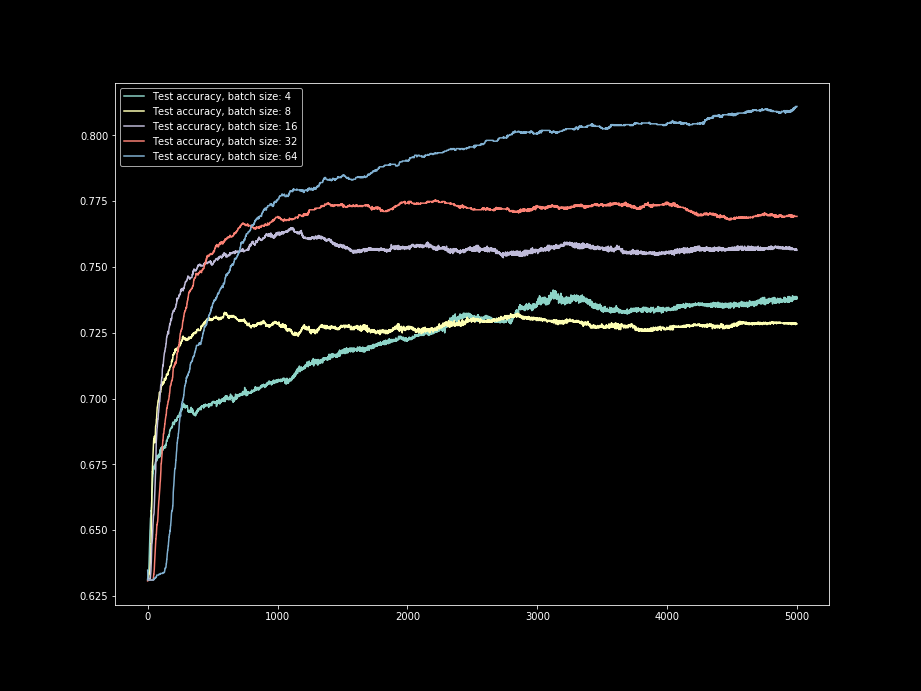
\includegraphics[width=0.8\linewidth]{assets/plots/part1_Q2a_3.png}
        \caption{Testing accuracy for different batch sizes}
        \label{fig:test_batch}
    \end{subfigure}
\caption{Batch size accuracies}
\label{fig:2a}
\end{figure}

Figure \ref{fig:2a} shows the results obtained from different batch sizes. Figure \ref{fig:2_1a} shows the time that different batch sizes operates per epoch.

\subsubsection{Part B}
From Figure \ref{fig:test_batch}, it can be seen that the accuracy of the curve with a batch size of 64 gives a better overall accuracy than all the other batch sizes.

\subsubsection{Part C}

\begin{figure}[H]
    \centering
    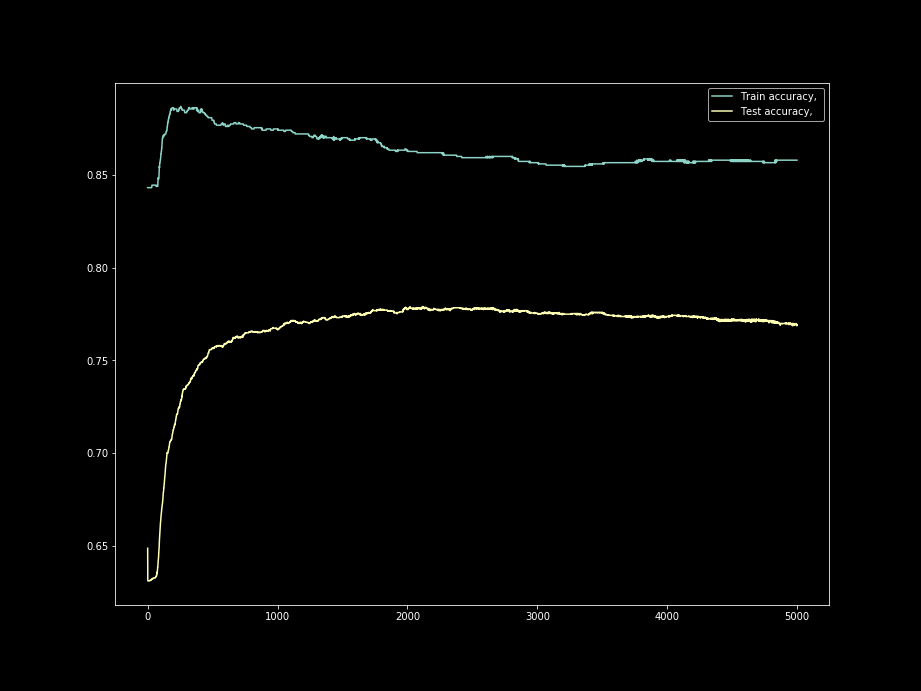
\includegraphics[width=0.8\linewidth]{assets/plots/part1_Q1a.png}
    \caption{Plot of training and testing data of optimal batch size of 64 against epochs}
    \label{fig:2c}
\end{figure}

Figure \ref{fig:2c} shows the train and test accuracies against epochs for the optimal batch size of 64.

\subsection{Question 3}
\label{1q3}
\begin{quote}
3. Find the optimal number of hidden neurons for the 3-layer network designed in part (2).

a) Plot the cross-validation accuracies against the number of epochs for different number of hidden-layer neurons. Limit the search space of number of neurons to {5,10,15,20,25}.

b) Select the optimal number of neurons for the hidden layer. State the rationale for your selection.

c) Plot the train and test accuracies against epochs with the optimal number of
neurons.
\end{quote}
\subsubsection{Part A}

\begin{figure}[H]
    \begin{subfigure}{1\textwidth}
        \centering
        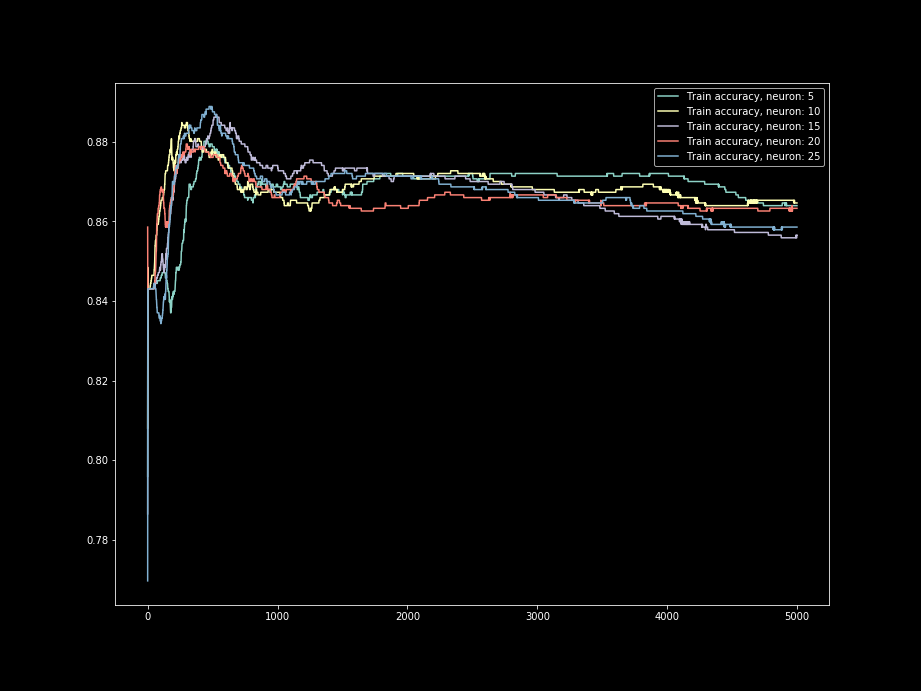
\includegraphics[width=0.8\linewidth]{assets/plots/part1_Q3a_3.png}
        \caption{Training accuracy for different neuron sizes}
        \label{fig:train_neuron}
    \end{subfigure}
\end{figure}
\begin{figure}[H]
    \ContinuedFloat
    \begin{subfigure}{1\textwidth}
        \centering
        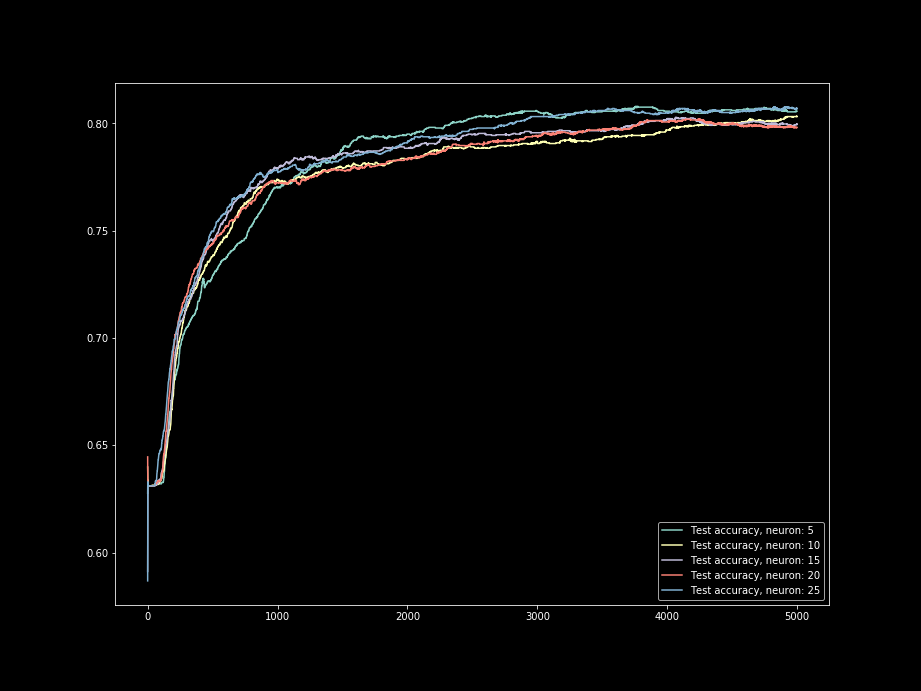
\includegraphics[width=0.8\linewidth]{assets/plots/part1_Q3a_2.png}
        \caption{Testing accuracy for different neuron sizes}
        \label{fig:test_neuron}
    \end{subfigure}
    \caption{Accuracy for different neuron sizes}
    \label{fig:neuron}
\end{figure}

Figure \ref{fig:neuron} shows the accuracies obtained from both the test and train sets for neuron sizes of [5,10,15,20,25].

\subsubsection{Part B}
With reference to Figure \ref{fig:test_neuron}, it can be seen that a neuron size of 5 and 25 gives the best accuracy. However, the optimal number of neurons should be 5 as the complexity of the model will be lower. While both neuron size 5 and 25 gives approximately similar results, a lower complexity offered by neuron size 5 will ensure that the chances of a wrongly weighted weight is less likely. This will prevent accuracy loss in datasets introduced that are more different than those used in training and testing.

\subsubsection{Part C}

\begin{figure}[H]
    \centering
    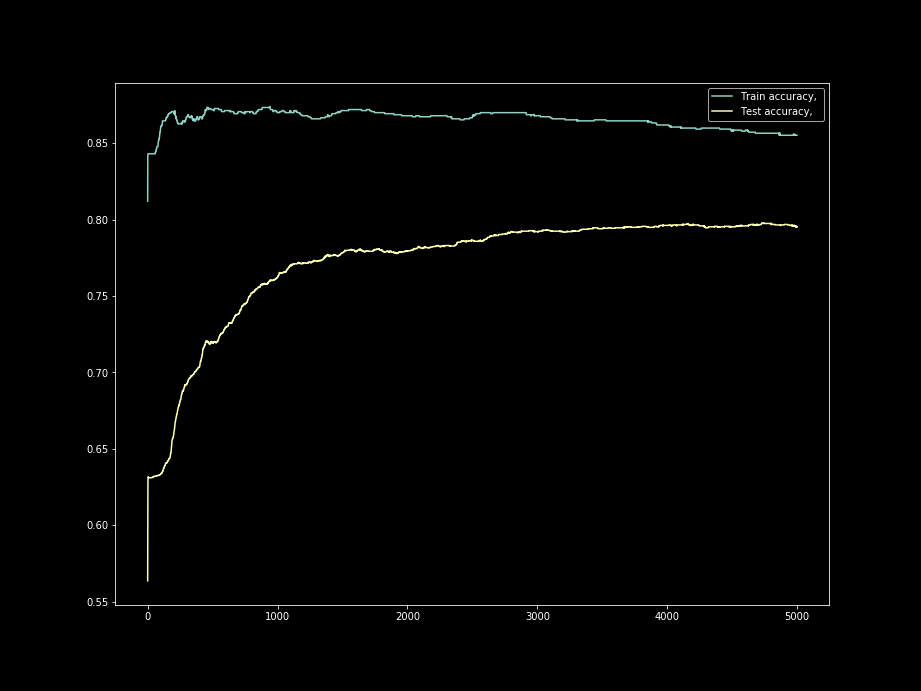
\includegraphics[width=0.8\linewidth]{assets/plots/part1_Q3c.png}
    \caption{Plot of training and testing data of optimal neuron size of 5 against epochs}
    \label{fig:3c}
\end{figure}

Figure \ref{fig:3c} shows the plot of training and testing data of optimal neuron size of 5 against epochs.

\subsection{Question 4}
\label{1q4}
\begin{quote}

4. Find the optimal decay parameter for the 3-layer network designed with optimal hidden neurons in part (3).

a) Plot cross-validation accuracies against the number of epochs for the 3-layer network for different values of decay parameters. Limit the search space of decay parameters to $[0, 10^-3, 10^-6, 10^-9, 10^-12]$.

b) Select the optimal decay parameter. State the rationale for your selection.

c) Plot the train and test accuracies against epochs for the optimal decay parameter.
\end{quote}
\subsubsection{Part A}

\begin{figure}[H]
    \begin{subfigure}{1\textwidth}
        \centering
        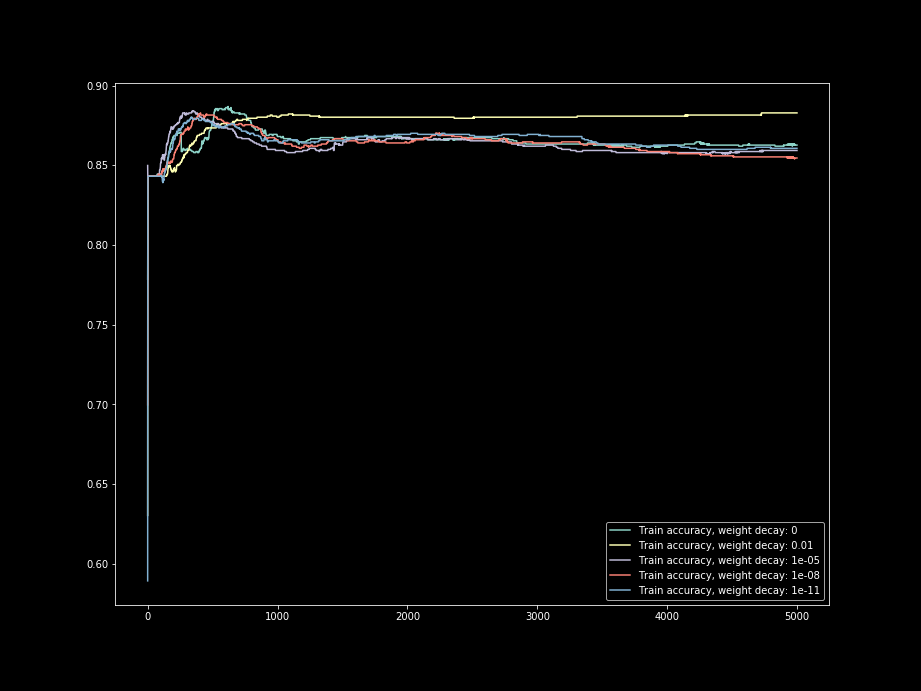
\includegraphics[width=0.8\linewidth]{assets/plots/part1_Q4a_3.png}
        \caption{Training accuracy for different decay parameters}
        \label{fig:train_decay}
    \end{subfigure}
\end{figure}
\begin{figure}[H]
    \ContinuedFloat
    \begin{subfigure}{1\textwidth}
        \centering
        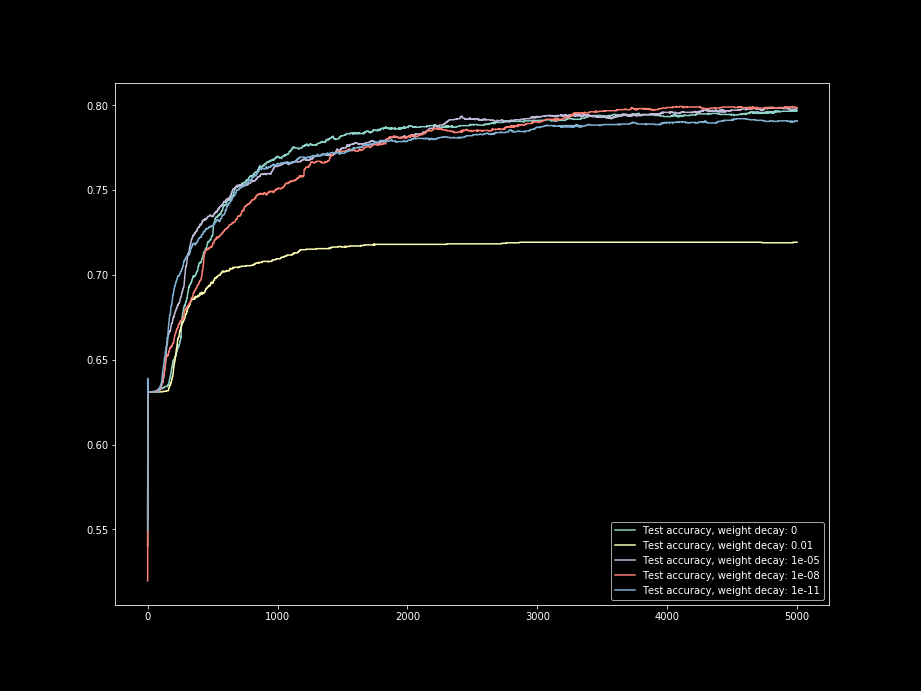
\includegraphics[width=0.8\linewidth]{assets/plots/part1_Q4a_2.png}
        \caption{Testing accuracy for different decay parameters}
        \label{fig:test_decay}
    \end{subfigure}
    \caption{Accuracy for different decay parameters}
    \label{decay}
\end{figure}

Figure \ref{decay} shows the result of the accuracies of the different weight decay parameters against epochs.

\subsubsection{Part B}

From Figure \ref{fig:test_decay}, it can be seen that the decay parameter of $10^{-9}$ performs the best as it has the best accuracy in the end. However, it is interesting to see that the decay parameter of $10^{-9}$ produced the best test accuracy despite not having the best training accuracy.

\subsubsection{Part C}
\begin{figure}[H]
    \centering
    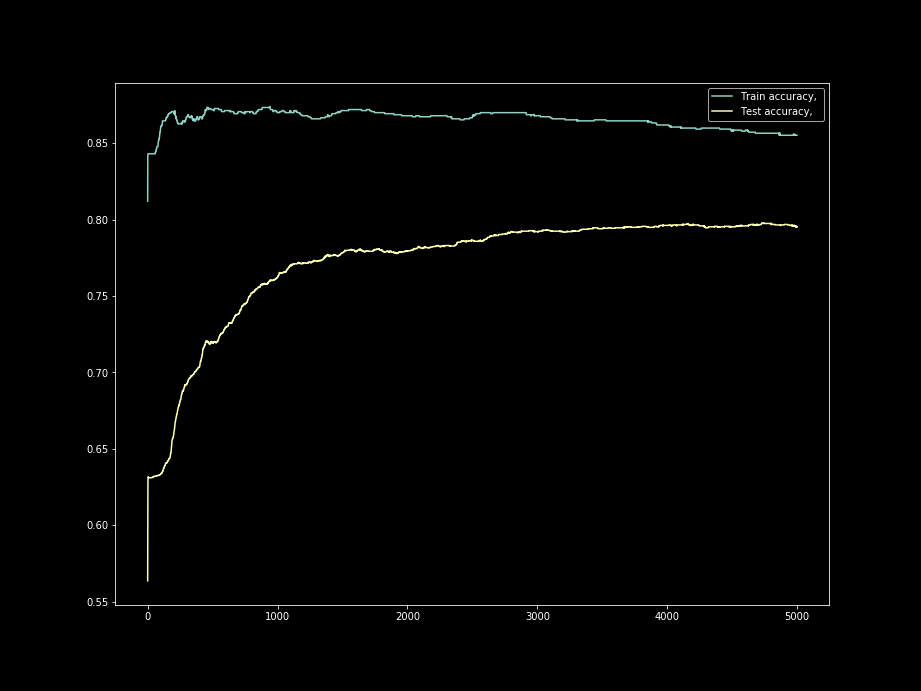
\includegraphics[width=0.8\linewidth]{assets/plots/part1_Q3c.png}
    \caption{Plot of training and testing data of optimal decay parameter of $10^{-9}$ against epochs}
    \label{fig:4c}
\end{figure}

Figure \ref{fig:4c} shows the plot of training and testing data of optimal decay parameter of $10^{-9}$ against epochs.

\subsection{Question 5}
\label{1q5}
\begin{quote}
5. After you are done with the 3-layer network, design a 4-layer network with two hidden layers, each consisting 10 neurons, and train it with a batch size of 32 and decay parameter $10^-6$.

a) Plot the train and test accuracy of the 4-layer network.

b) Compare and comment on the performances of the optimal 3-layer and 4-layer
networks
\end{quote}

The definition of the 4-layer network can be seen in Listing \ref{ls:1_l4}.

\begin{lstlisting}[language=Python, caption=4-layer feed forward network, label=ls:1_l4]
def l4_ffn(x, neuron_size, weight_decay_beta):
    """Feedforward net with 2 hidden layer.
    """
    sum_regularization = 0
    with tf.name_scope('hidden'):
        weights = tf.Variable(tf.truncated_normal([NUM_FEATURES, neuron_size], stddev=1.0/math.sqrt(float(NUM_FEATURES))), name='weights')
        biases  = tf.Variable(tf.zeros([neuron_size]), name='biases')
        h  = tf.nn.relu(tf.matmul(x, weights) + biases)
        sum_regularization += weight_decay_beta * tf.nn.l2_loss(weights)
    with tf.name_scope('hidden2'):
        weights = tf.Variable(tf.truncated_normal([neuron_size, neuron_size], stddev=1.0/math.sqrt(float(neuron_size))), name='weights')
        biases  = tf.Variable(tf.zeros([neuron_size]), name='biases')
        h  = tf.nn.relu(tf.matmul(h, weights) + biases)
        sum_regularization += weight_decay_beta * tf.nn.l2_loss(weights)
    with tf.name_scope('linear'):
        weights = tf.Variable(tf.truncated_normal([neuron_size, NUM_CLASSES], stddev=1.0/math.sqrt(float(neuron_size))), name='weights')
        biases  = tf.Variable(tf.zeros([NUM_CLASSES]), name='biases')
        u = tf.matmul(h, weights) + biases
        sum_regularization += weight_decay_beta * tf.nn.l2_loss(weights)
    
    return u, sum_regularization
\end{lstlisting}

\subsubsection{Part A}

\begin{figure}[H]
    \centering
    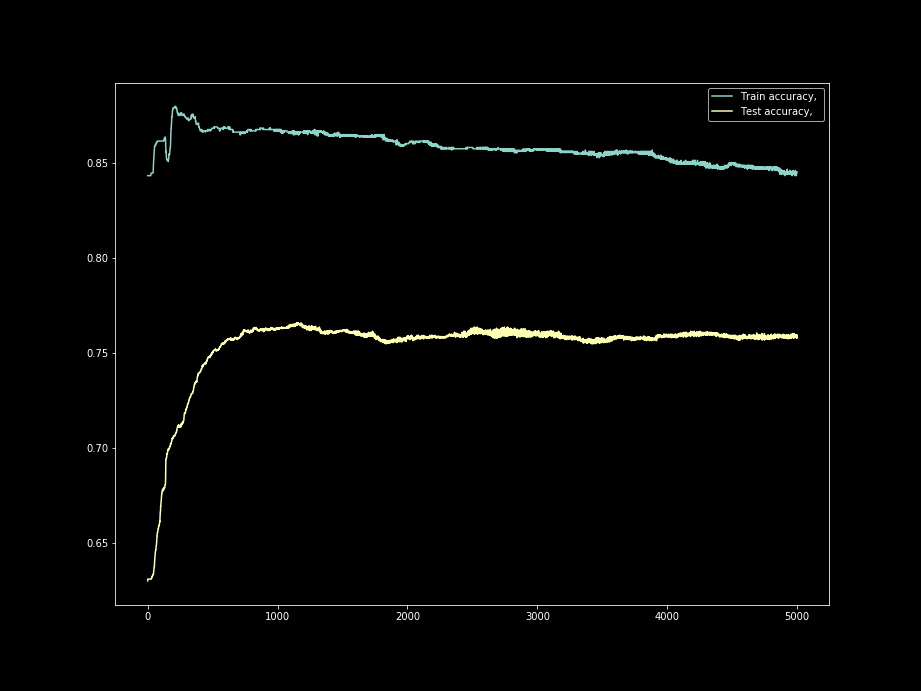
\includegraphics[width=0.8\linewidth]{assets/plots/part1_Q5a.png}
    \caption{Plot of training and testing data of a 4-layer network against epochs}
    \label{fig:5a}
\end{figure}

Figure \ref{fig:5a} shows the plot of training and testing data of a 4-layer network against epochs.

\subsubsection{Part B}

\begin{figure}[H]
    \begin{subfigure}{1\textwidth}
        \centering
        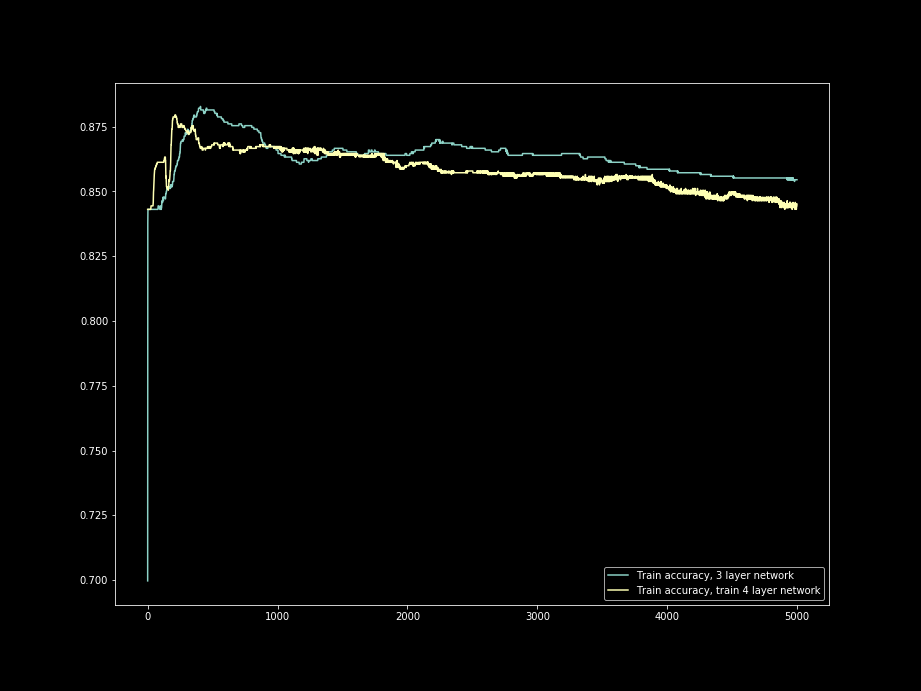
\includegraphics[width=0.8\linewidth]{assets/plots/part1_Q5b_3.png}
        \caption{Training accuracy for optimal 3-layer and 4-layer network}
        \label{fig:train_34}
    \end{subfigure}
\end{figure}
\begin{figure}[H]
    \ContinuedFloat
    \begin{subfigure}{1\textwidth}
        \centering
        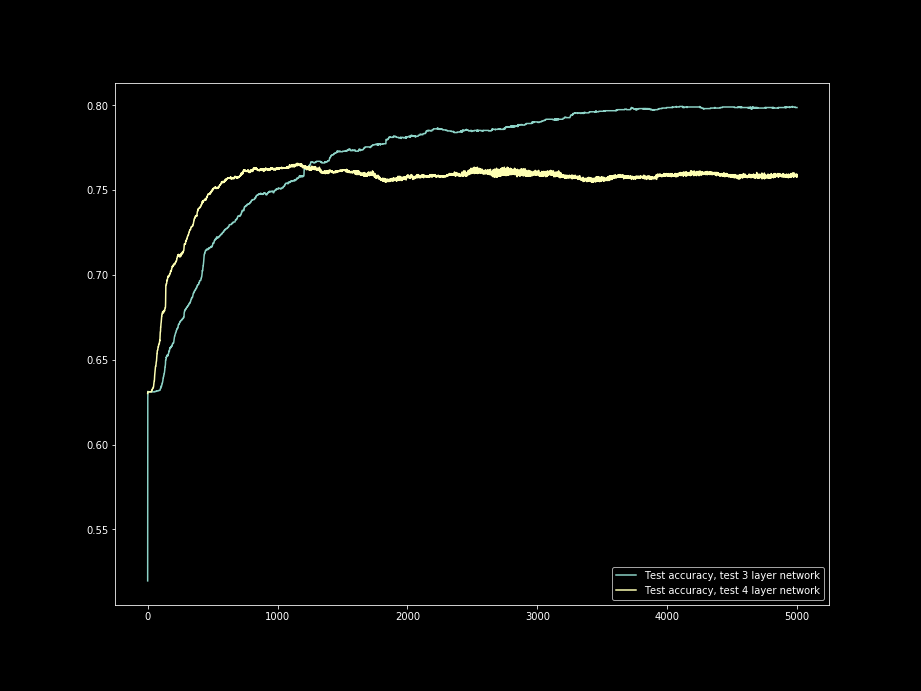
\includegraphics[width=0.8\linewidth]{assets/plots/part1_Q5b_2.png}
        \caption{Testing accuracy for optimal 3-layer and 4-layer network}
        \label{fig:test_34}
    \end{subfigure}
\end{figure}

As shown in Figure \ref{fig:train_34} \& \ref{fig:test_34}, we can see that the 3 layer network has better performance than 4 layer network. This may be due to having too many layers for the dataset when it is not really necessary, which could result in overfitting. This is shown in Figure \ref{fig:train_34}, as the train accuracy of the 4-layer network is almost the same as the 3-layer network, while in Figure \ref{fig:train_34}, there was a significant difference in the performance of them. As such, the performance of the 3-layer network in this dataset is better than the 4-layer network defined by the question.
